\documentclass[../../main.tex]{subfiles}

\begin{document}
\providecommand{\szz}{\mathcal{S}}
\providecommand{\ccinf}{C_c^\infty}

% Topologies
\providecommand{\Taux}{\Tau_\xx}
\providecommand{\Tauy}{\Tau_\yy}
\providecommand{\Tauxy}{\Tau_{\xx\times\yy}}

% Basis
\providecommand{\Bx}{\borel_\xx}
\providecommand{\By}{\borel_\yy}
\providecommand{\Bxy}{\borel_{\xx\times\yy}}


\section*{Notes on Chapter 4}

\topheader{Topological Spaces}

This section will roughly follow Munkres text on Geeneral Topology, in particular we hope to cover Chapters 2, 3, 4 and 9. The rest of the Chapters should be covered proper by the subsequent section.


\begin{definition}[Topology]\label{chp4:topology-definition}
    Let $\xx$ be a non-empty set. A topology $\Tau$ on $\xx$, sometimes denoted by $\Tau_\xx$ is a family of subsets of $\xx$, 
\begin{itemize}
    \item $\{\varnothing,\xx\}\subseteq \Tau$,
    \item If $U_1$ and $U_2$ are elements of $\Tau$, so is their intersection.
    \item If $\{U_\alpha\}$ is an arbitrary family of sets in $\Tau$, their union is also contained in $\Tau$ as an element.
\end{itemize}
We call the elements of $\Tau$ open sets. The complements of elements in $\Tau$ are closed sets.
\end{definition}

\newpage


\topheader{Basis of a Topology}

\begin{definition}[Basis of a topology]\label{chp4:basis-definition}
    A basis $\borel$ is a family of subsets of $\xx$, that satisfies:
    \begin{itemize}
        \item Every $x\in\xx$ belongs (as an element) in some $V\in\borel$.
        \item If $B_1$ and $B_2$ are basis elements, such that their intersection is non-empty. Then every $x\in B_1\cap B_2$ induces a $B_3\in\borel$ with 
        \[
            x\in B_3\subseteq B_1\cap B_2
        \]
    \end{itemize}
    This roughly means a basis is 'finitely' fine at every point in $x$.
\end{definition}

If $\borel$ is a basis, it 'generates' a topology $\Tau$ through

\begin{equation}\label{chp4:basis-generates-topology}
    \Tau = \bigset{U\subseteq\xx,\: \forall x\in U,\: x \in B\subseteq U \text{ for some } B \in \borel}
\end{equation}

Notice this is equivalent to $\Tau$ is the collection of all unions of basis elements in $\borel$.

\begin{wts}
    Let $\borel$ be a basis as defined in \Cref{chp4:basis-definition}, then $\Tau$ as defined in \Cref{chp4:basis-generates-topology} is a valid topology on $\xx$. And every member of $\Tau$ is and is precisely the union of elements in $\borel$.
\end{wts}
\begin{proof}
    Every point in $\xx$ belongs in some basis element, so $\xx\in\Tau$, so does $\varnothing$. Next, if $U_1$ and $U_2$ are in $\Tau$, then 
    \[
        \begin{cases}
            x\in U_1\induces x\in B_1\subseteq U_1\\
            x\in U_2\induces x\in B_2\subseteq U_2\\
        \end{cases}\implies x\in B_3\subseteq B_1\cap B_2\subseteq U_1\cap U_2
    \]
    for some $B_3\in\borel$, so $\Tau$ is closed under finite intersections (perhaps after a standard induction argument).\\

    If $\{U_\alpha\}\subseteq \Tau$, and $x$ belongs in the union of all $U_\alpha$, then $x\in B_\alpha\subseteq U_\alpha$, which is a subset of the entire union. So the union over $U_\alpha$ is again contained in $\Tau$, and $\Tau$ is a topology on $\xx$.\\

    It is worth noting that $\borel\subseteq\Tau$. Finally, if $U\in\Tau$, 
    \[
        U = \bigcup_{x\in U}B_x
    \]
    where $B_x$ is the basis element taken to satisfy $x\in B_x\subseteq U$. Every point in $U$ is included in some $B_x$, and hence is included in the union. For the reverse inclusion, notice the union of subsets of $U$ is again a subset of $U$. \\
    
    Now, if $E\subseteq\xx$ is the union of basis elements in $\borel$, if $E$ is non-empty, then every point $x\in E$ belongs in some $B_x$. Recycling the previous argument, and we see that $E$ is open in $\Tau$. If $E$ is empty, we define the 'union' of no sets as the empty set. So $\Tau$ is precisely the collection of all unions of basis elements $\borel$.
\end{proof}
\newpage

We are now in a position to compare the relative 'fineness' of topologies.

\begin{definition}[Fineness of topologies]\label{chp4:finer-toplogies}
    If $\Tau'$ and $\Tau$ are both topologies on some non-empty set $\xx$. We say $\Tau'$ is finer than $\Tau$, or $\Tau$ is coarser than $\Tau'$ if 
    \[
        \Tau'\supseteq \Tau
    \]
\end{definition}

\begin{wts}\label{chp4:basis-finer-topology-finer}
    If $\borel$ and $\borel'$ are bases for $\Tau'$ and $\Tau$, the following are equivalent:
    \begin{itemize}
        \item $\Tau'$ is finer than $\Tau$,
        \item If $B$ is an arbitrary basis element in $\borel$, then every point $x\in B$ induces a basis element in $\borel'$ with
        \[
            x\in\borel'\subseteq\borel
        \]
    \end{itemize}
\end{wts}
\begin{proof}
    Suppose $\Tau'$ is finer than $\Tau$. Notice $\borel\subseteq\Tau'$ as well. By \Cref{chp4:basis-generates-topology}, each $x\in B$ induces a $B'\in\borel'$
    \[
        x\in B'\subseteq B
    \]
    Conversely, fix any open set $U\in\Tau$, and for each $x\in U$, 
    \[
        x\in B'\subseteq B\subseteq U
    \]
    Applying \Cref{chp4:basis-definition} tells us $U$ is open in $\Tau'$.
\end{proof}
\newpage

The last of the big three 'generating' definitions for topologies will be the sub-basis. It simply means the first condition (but not necessarily) the second, is satisfied in \Cref{chp4:basis-definition}
\begin{definition}[Sub-basis of a topology]\label{chp4:sub-basis-definition}
    A sub-basis $S\in\powerset{\xx}$ is a family of subsets of $\xx$ that satisfies one property. Any point $x$ in $\xx$ belongs to at least one member of $S$.
\end{definition}
A sub-basis can be upgraded to a basis by collecting all of its finite intersections.
\begin{wts}
    Let $S$ be a sub-basis of $\xx$, then the collection of all finite intersections of $S$ forms a basis $\borel$ of $\xx$.
\end{wts}
\begin{proof}
    Every point in $\xx$ lies in some element of $S$, hence in some element of $\borel$. The second basis property is immediate, since $\borel$ is closed under finite intersections.
\end{proof}
\newpage

\topheader{Product Topology}
We will start with products of a finite collection of topological spaces.
\begin{definition}[Finite Product of Topological Spaces]\label{chp4:finite-product-topology}
    Let $(\xx,\Tau_\xx)$ and $(\yy,\Tau_\yy)$ be topological spaces. The product topology (denoted by $\Tauxy$) on $X\times Y$ is defined as the topology generated by the basis

    \begin{equation}\label{chp4:finite-product-basis}
        \borel_{\xx\times \yy} = \bigset{U\times V,\: (U, V)\in \Tau_\xx\times \Tau_\yy}
    \end{equation}
\end{definition}
Since bases are easier to describe than topologies, we have the following statement concerning the basis of the product topology.
\begin{wts}
    If $\Bx$ and $\By$ are bases for $\Taux$ and $\Tauy$, then the product topology (as described in \Cref{chp4:finite-product-topology}) is also generated by
    \begin{equation}\label{chp4:finite-product-basis2}
        \mcal = \bigset{U\times V,\: (U,V)\in\Bx\times \By}
    \end{equation}
\end{wts}
\begin{proof}
    We will introduce (and use) the technique of 'double inclusion' by proving that the topologies generated are both finer than the other. Let us denote the topology generated by $\mcal$ in \Cref{chp4:finite-product-basis2} by $\Tau_\mcal$.\\
    
    Since $\Bx\times\By\subseteq\Taux\times\Tauy$, if $U\times V\in \mcal$ as in \Cref{chp4:finite-product-basis2}, then we can pick the same 'open rectangle' again. We trivially have
    \[
        x\in \underbrace{U\times V}_{\text{member of } \Taux\times\Tauy}\subseteq U\times V
    \]
    and by \Cref{chp4:basis-finer-topology-finer}, $\Tauxy$ is finer than $\Tau_\mcal$.\\

    Fix any set $U\times V\in\Bxy$, and if $(p,q)\in U\times V$, each coordinate induces basis elements from $\Bx$ and $By$, more precisely:
    \[
        \begin{cases}
            p\in U\implies p\in \text{Basis element of } \Bx\subseteq U\\
            q\in V\implies q\in \text{Basis element of } \By\subseteq V\\
        \end{cases}\implies (p,q)\in \underbrace{\:}_{\text{ in }\Bx}\times \underbrace{\:}_{\text{ in }\By}\subseteq U\times V
    \]
    by \Cref{chp4:basis-finer-topology-finer}, $\Tau_\mcal$ is finer than $\Tauxy$ and $\Tauxy = \Tau_\mcal$.
\end{proof}





\newpage

\topheader{Quotient Topology}




\newpage

\topheader{Product Topology}

The Cartesian Product of an arbitrary family of topological spaces, if equipped with the product topology, preserves a lot of the structure. If $\{X_\alpha\}_{\alpha\in A}$ is a family of topological spaces which are $\rule{1cm}{0.15mm}$, then $\prod X_\alpha$ is $\rule{1cm}{0.15mm}$. Replace $\rule{1cm}{0.15mm}$ with: 

\begin{enumerate}
    \item Hausdorff, (Folland)
    \item Regular,
    \item Connected, (Munkres chp23, exercise 10)
    \item First countable, if $A$ is countable,
    \item Second countable, if $A$ is countable,
    \item Compact (Tynchonoff's Theorem, Folland)
\end{enumerate}

\newpage

\topheader{Connectedness}

\begin{definition}[Connectedness]\label{chp4:connectedness-definition}
    A topological space $\xx$ is connected if $U$ and $V$ are disjoint open subsets whose union is $\xx$, then at least one of $U$ or $V$ is empty.
\end{definition}
See Folland Exercise 4.10 for more properties.

\begin{definition}[Path-connectedness]\label{chp4:path-connectedness-definition}
    A topological space $\xx$ is path-connected if for any two pair of points $x$, $y\in\xx$. There exists a continuous function $f:[a,b]\to \xx$, with $f(a)=x$ and $f(b)=y$.
\end{definition}

\begin{definition}[Connected component]\label{chp4:connected-component-definition}
    The connected components of $\xx$ is the family of equivalence classes on $\xx$, where $x\sim y$ if there is a connected subspace of $\xx$ that contains both of them.
\end{definition}


\begin{wts}
    Continuous functions map connected spaces to connected spaces (in the subspace topology).
\end{wts}
\begin{proof}
    Let $\xx$ and $\yy$ be topological spaces and $f: \xx\to\yy$ be continuous. If $f(\xx)$ is disconnected, then we can find $U$ and $V$, open and disjoint in $\Tau_{f(\xx)}$ such that
    \[
        U\cup V = f(\xx)\implies f^{-1}(U)\cup f^{-1}(V) = \xx
    \]
    where $f^{-1}(f(\xx)) = \xx$. Both $f^{-1}(U)$ and $f^{-1}(V)$ are open, non-empty, and are pairwise disjoint. So $\xx$ is separated.
\end{proof}

\begin{wts}
    Let $(\xx_\alpha,\: \Tau_{\alpha})$ be a family of connected topological spaces indexed by $\alpha\in A$. Then $\prod_{\alpha\in A}\xx_\alpha$ is disconnected in the product topology.
\end{wts}
\begin{proof}
    We will attempt the contrapositive. Suppose $\prod_{\alpha\in A}\xx_\alpha$ is disconnected, then
\end{proof}



\newpage
\subsection*{Topology in Analysis}
\topheader{Interiors and closures}
\begin{definition}[Interior of a set]\label{chp4:interior-definition}
    $A^o$ is defined to be the largest open subset of $A$, 
    \[
        A^o = \bigcup_{\mathclap{\substack{\text{$U$ open, }\\ U\subseteq A}}} U
    \]
\end{definition}
\begin{corollary}\label{chp4:interior-subset}
    The union of subsets of $A$ is again a subset of $A$, therefore \Cref{chp4:interior-subset} implies $A^o\subseteq A$ for any $A\subseteq \xx$. 
\end{corollary}

%%%%

\begin{definition}[Closure of a set]\label{chp4:closure-definition}
    and $\cl{A}$ is the smallest closed superset of $A$,
    \[
        \cl{A} = \bigcap_{\mathclap{\substack{\text{$K$ closed, }\\ A\subseteq K}}} K
    \]
\end{definition}


%%%%
\begin{wts}\label{chp4:flipping-interior-to-closure}
    The complement of the closure is the interior of the complement, or equivalently: $(\cl{A})^c = A^{co}$
\end{wts}
\begin{proof}
    Taking complements, and the substitution $U = K^c$ reads
    \begin{align*}
        (\cl{A})^c &= \biggl[\bigcap_{{\substack{\text{$K$ closed, }\\ A\subseteq K}}} K \biggr]^c\\[2ex]
        &= \bigcup_{\mathclap{\substack{\text{$K$ closed, }\\ K^c\subseteq A^c}}} K^c\\[2ex]
        &= \bigcap_{\mathclap{\substack{\text{$U$ open, }\\ U\subseteq A^c}}} U\\[2ex]
        &= A^{co}
    \end{align*}
\end{proof}
\begin{remark}
    Personally, I remember this as pushing the complement inside and flipping the bar to a $c$!
\end{remark}

\newpage
\topheader{Neighbourhoods}
The concept of a neighbourhood allows us to characterize the interior of a set 'locally'.
% Neighbourhoods, use Folland Definition
\begin{definition}[Neighbourhood (not necessarily open)]\label{chp4:neighbourhood-definition}
    A neighbourhood of $x\in\xx$ is a set $U\subseteq\xx$ where $x\in U^o$. The set of neighbourhoods for a point $x\in\xx$ will sometimes be denoted by $\N(x)$.
\end{definition}
\begin{wts}[Characterization of the interior]
    If $W = \bigset{x\in\xx, \: \text{there exists a neighbourhood $U$ of $x$,}\: U\subseteq A}$, then $W = A^o$.
\end{wts}
\begin{proof}
    If $x\in A^o$, then $A$ is a neighbourhood of $x$, and $A\subseteq A$, so $x\in W$. Conversely, if $x$ is a member of $W$, it has a neighbourhood $U\subseteq A$ (not necessarily open). By monotonicity of the interior,
    \[
        x\in U^o\subseteq A^o
    \]
    and $x\in A^o$.
\end{proof}
It is easy to see that $A$ is open $\iff A^o = A \iff A$ is a neighbourhood of itself. 
\begin{itemize}
    \item The first equivalence follows from:
    \[
        E\subseteq\xx\implies E^o\subseteq E
    \]
    and if $A$ is an open set, it is an open subset of itself, by \Cref{chp4:interior-subset} $A\subseteq A^o$. If $A^o = A$, then it suffices to show that $A^o$ is open. Which it is, since it is the arbitrary union of open sets.
    \item To prove the second equivalence: suppose $A^o = A$, then each $x\in A$ has a neighbourhood contained (as a subset) in $A$, namely $A$ itself. (This statement is hard to parse, the reader is encouraged to really work through this and be honest).
    \[
        x\in A^o\subseteq A\implies A\subseteq A^o
    \]
    so $A$ is a neighbourhood of itself. Conversely, if $A\subseteq A^o$, then $A = A^o$, since the reverse inclusion follows immediately from \Cref{chp4:interior-subset}.
\end{itemize}

\newpage
\topheader{Adherent points}
Similar to the neighbourhood, the concept of an adherent point of a set allows us to speak of the closure in more concrete terms. The following definition is key in understanding the relationship between the closure, interior, and the boundary.
\begin{definition}[Adherent point of a set]\label{chp4:adherent-point-definition}
    Let $A\subseteq\xx$, $x\in\xx$ is an adherent point of $A$ if every neighbourhood $U$ of $x$ intersects $A$. In symbols,
    \[
        U\cap A\neq\varnothing,\quad\forall U\in\N{x}
    \]
\end{definition}
\begin{wts}[Characterization of the closure]\label{chp4:closure-adherent}
    Let $A\subseteq X$, and let $W$ be the set of adherent points of $A$, then $\cl{A}=W$
\end{wts}
\begin{proof}
    Suppose $x\notin W$, then there exists a neighbourhood $U$ of $x$ where
    \[
        U\cap A=\varnothing\iff U\subseteq A^c
    \]
    this is exactly the definition of the interior of $A^c$, so $x\in A^{co}$ and recall (from \Cref{chp4:flipping-interior-to-closure}) that $(\cl{A})^c = A^{co}$, so $x\notin \cl{A}$. For the reverse inclusion, read the proof backwards, by flipping $\forall\to\exists$ within the set, and we see that
    \[
        W^c = A^{co} = (\cl{A})^c
    \]
\end{proof}

\newpage

\topheader{Dense and nowhere dense subsets}
\begin{definition}[Dense subset]\label{chp4:dense-definition}
    A subset of a topological space $E\subseteq\xx$ is dense if $\cl{E} = \xx$.
\end{definition}

\begin{definition}[Nowhere dense subset]\label{chp4:nowhere-dense-definition}
    A subset of a topological space $E\subseteq\xx$ is nowhere dense if $\cl{E}^o = \varnothing$.
    
    This means $E$ is dense in none of the (non-trivial) open subspaces of $\xx$.
\end{definition}

\begin{wts}\label{chp4:dense-equivalences}
    $E$ is dense in $\xx$ iff for every non-empty, open set $U\subseteq\xx$, $U\cap E\neq\varnothing$.
\end{wts}
\begin{proof}[Proof of \Cref{chp4:dense-equivalences}]
    Suppose $E$ is dense, then $\cl{E}=\xx$. Every point of $\xx$ is an adherent point of $E$. Let $U\subseteq \xx$ be a non-empty open set. If $x\in U$ then $U$ is a neighbourhood of $x$, thus $U$ intersects $E$. Conversely, suppose every non-empty open set $U$ intersects $E$. Fix any point $x\in\xx$, and any neighbourhood $U$ of $x$. $U$ has a non-empty interior (because it must contain $x$). But $U^o$ is a non-empty open set, therefore $\varnothing\neq U^o\cap E\subseteq U\cap E$
\end{proof}

\begin{wts}\label{chp4:nowhere-dense-homeomorphisms}
    Let $f:\xx\to\xx$ be a homeomorphism. $E$ is nowhere dense iff $f(E)$ is nowhere dense.
\end{wts}
\begin{proof}
    Since $f^{-1}$ is a homeomorphism, suppose $\cl{f^{-1}(E)}^o\neq\varnothing$, there exists a non-empty, open subset $U\subseteq\xx$ with
    \[
        \cl{f^{-1}(E)}\cap U = U
    \]
    The direct image yields 
    \[
        f\biggl((\cl{f^{-1}(E)})\cap U\biggr) = f(U)
    \]
    since $f$ is a bijection (injectivity is necessary here), it commutes with intersections.
    \begin{equation}\label{chp4:nowhere-dense-direct-image}
        f(\cl{f^{-1}(E)})\cap f(U) = f\biggl((\cl{f^{-1}(E)})\cap U\biggr) = f(U)
    \end{equation}
    and $f$ is continuous, so $f(\cl{A})\subseteq\cl{f(A)}$ for any $A\subseteq\xx$. For the reverse inclusion, $f$ is a closed map, so $f(\cl{A})$ is a closed superset of $f(A)$ so 
    \[
        f(\cl{A}) = \cl{f(A)}
    \]
    Take $A = f^{-1}(E)$, and $f(\cl{f^{-1}(E)}) = \cl{f(f^{-1}(E))} = \cl{E}$. From \cref{chp4:nowhere-dense-direct-image}, we see that
    \[
        \cl{E}\cap f(U) = f(U)
    \]
    $f(U)$ is a non-empty open subset of $\xx$, since $f$ is an open map, so $E$ is not no-where dense. The reverse implication can be proven by replacing $f$ with $f^{-1}$.
\end{proof}


\newpage


\topheader{Urysohn's Lemma Notes}
Notes on the construction of the countable 'onion' sequence within a normal space $\xx$.\\

If $\xx$ is a normal space, and $A$ and $B$ are disjoint closed subsets, then we can easily find an open $U$ with
\begin{equation}\label{eq:UrysohnLemma-Seashells}
    A\subseteq U \subseteq \cl{U}\subseteq B^c
\end{equation}
We say that $U$ hides in $B^c$ if the closure of $U$ is contained in $B^c$. Define $\Delta_n = \bigset{k2^{-n},\: 1 < k < 2^{n}}$, so that $\Delta_n\subseteq(0,1)$ for all $n\geq 1$. Notice 
\[
    \Delta_1\supseteq \cdots\supseteq \Delta_n\supseteq \Delta_{n+1}
\]
and the even indices for $\Delta_{n+1}$ are contained in $\Delta_n$. Suppose $\Delta_n$ is well defined, it suffices to choose the odd indices for $\Delta_{n+1}$. If $r = j2^{-(n+1)}$, where $j$ is odd, then $r$ sits in between precisely two elements in $\Delta_n\cup\{0,1\}$. If $r$ sits between an endpoint, then define $\cl{U_0} = A$, and $B^c = U_1$. And denote the closest left and neighbours by $s$, $t$ respectively. If $s<r<t$, it is clear that $\cl{U_s}$ and $U_t^c$ are disjoint closed sets.\\

Use the 'normal space' construction to obtain an superset of $\cl{U_s}$ that hides in $U_t$, denote this open set by $U_r$, and similar to \Cref{eq:UrysohnLemma-Seashells}
\[
    \cl{U_s}\subseteq U_r\subseteq \cl{U_r}\subseteq U_t
\]
Now that the construction of this sequence is complete, we wish to prove Urysohn's Lemma. Let $A$ and $B$ be disjoint closed sets. And define 
\[
    f(x) = \inf\bigset{r\in\Delta\cup\{1\},\: x\in U_r}
\]
where $U_1 = \xx$. So that $0\leq f(x)\leq 1$ is immediate. If $x\in A$, then $x$ is in all $U_r$, and by density of $\Delta\subseteq(0,1)$, we have $f(x)=0$. Conversely, if $x\in B$ then $x\notin U_r$ for all $r\in\Delta$, if $E$ denotes the indices in $\Delta$ where $x\in U_s$ when $s\in E$,
\begin{equation}\label{inequality shortcut infimum intervals}
    (-\infty,\: r)\subseteq E^c\iff E\subseteq [r,\: +\infty)\iff\inf(E)\geq r
\end{equation}
Send $r\to 1$ and $f(x) = 1$. Thus $f|_{A}=0$ and $f|_{B}=1$.\\

To show continuity, it suffices to show that the inverse images of the open half $\bigset{(x > \alpha),\: (x < \alpha)}_{\alpha\in\real}$ lines are indeed open in $\xx$. Let $\alpha$ be fixed. And if $x\in \{f<\alpha\}$, we can 'wiggle' the infimum towards the right (towards $\alpha$), and using density of $\Delta$ within $(0,1)$, there exists a $r\in E$ that satisfies $f(x) < r < \alpha$. This is equivalent to 
\[
    x\in \bigcup_{r<\alpha} U_r
\]
If there exists an $r<\alpha$ st $x$ belongs to $U_r$ as an element, then $f(x)\leq r < \alpha$.\\

If $f(x) > \alpha$, then $(-\infty,\: \alpha)\subseteq E^c$, by  \Cref{inequality shortcut infimum intervals}. Suppose $\alpha<1$, otherwise $\{f>\alpha\}=\varnothing$. Wiggle $f(x)$ to the left and obtain an $r\in\Delta$, $\alpha<r<f(x)$ with $x\notin U_r$. By density again, take any $s<r$ by a small amount (st $s>\alpha$, $s\in \Delta$), and
\[
    \cl{U}_s\subseteq U_r\iff U_r^c\subseteq\cl{U}_s
\]
so that $x\in \cl{U}_s^c$ for some $s>\alpha$. This is equivalent to 
\[
    x\in\bigcup_{s>\alpha}\cl{U}_s^c
\]
Conversely, if $x\notin \cl{U}_s^c$ for some $s>\alpha$,  since $\{U_r\}$ (thus $\{\cl{U}_r\}$) is increasing, and $x\notin U_r$ for every $r\leq s$. Hence,
\[
    (-\infty,\: s]\subseteq E^c\iff E\subseteq (s,\: +\infty)\iff f(x)\geq s>\alpha
\]

\newpage
\topheader{Compactness}
Compactness is one of the most important concepts in topology and analysis.

\begin{definition}[Compact topological space]\label{chp4:compact-space-definition}
    A topological space $\xx$ is compact if every open covering $\{U_\alpha\}$ contains a finite subcover. That is, if $\{U_\alpha\}$ is an arbitrary collection of open sets, then
    \[
        \xx  = \bigcup U_{\alpha\in A}\implies\bigcup_{j\leq n}U_{\alpha_j}
    \]
\end{definition}

\begin{definition}[Compact set]\label{chp4:compact-set-definition}
    $E\subseteq\xx$ is compact if it is compact in the subspace topology.
\end{definition}

\begin{definition}[Precompact set]\label{chp4:precompact-set-definition}
    $E\subseteq\xx$ is precompact if its closure is compact (as a subset).
\end{definition}

\begin{definition}[Paracompact space]\label{chp4:paracompact-set-definition}
    A topological space $\xx$ is paracompact if every open covering of $\xx$ has a locally finite open refinement that covers $\xx$.
\end{definition}

\begin{definition}[Locally finite collection of sets]\label{chp4:locally-finite-definition}
    Let $\acal$ be a collection of subsets of $\xx$. It is called locally finite, if at every point $p\in \xx$, we can find a neighbourhood $U$ of $p$ (not necessarily open), that intersects only finitely many members of $\acal$. In symbols,
    \[
        U\cap E=\varnothing\qq{for all but finitely many}E\in\acal
    \]
    We do not require $\acal$ to be a cover of $\xx$, nor do we require $\acal$ to be a collection of open sets.
\end{definition}

\begin{definition}[Countably locally finite]\label{chp4:countably-locally-finite-definition}
    A collection $\borel$ is countably locally finite if it is the countable union of locally finite families.
    \[
        \borel = \overbracket{\bigcup_{\nat}}^{\mathclap{\substack{\text{countable}\\ \text{union}}}}\borel_n,\quad\text{where each }\borel_n\text{ is a locally finite collection}
    \]
\end{definition}
    
\begin{definition}[Refinement]\label{chp4:refinement-definition}
    If $\acal$ is a collection of sets, $\borel$ is a refinement of $\acal$ if every element $B\in\borel$, induces an element $A\in\acal$, such that $B\subseteq A$.
\end{definition}
\begin{remark}[Intuition for refinements]
    If $\borel$ is a refinement of $\acal$, we can use the 'absolute continuity' muscle. For each element in $\borel$ is dominated by some element (through subset inclusion) in $\acal$. Recall, if $\nu$ and $\mu$ are non-negative measures, then $\nu\ll\mu$ if for every measurable set $E\in\mcal$, $\mu(E)=0\implies \nu(E)=0$.\\
    
    A refinement of a family of sets is another family of sets, whose elements are dominated by some other element in the un-refined family. \emph{Refining families makes them 'smaller', cover less area.}
\end{remark}


\newpage

\topheader{Locally Compact Hausdorff Spaces}
Compactness is an intrinsic topological property (in the subspace topology). We see from Proposition 4.25 that compact Hausdorff spaces are normal, which gives a sufficient condition for us to approximate and extend any continuous function; and allows us to extend certain 'local' properties to 'global' properties. \\

If given a Hausdorff space, not necessarily compact, the natural question is to ask 1) whether a topological space has 'enough' compact subsets to work with, and 2) whether we can embed a given topological space in a larger one to force it to be compact.

\begin{definition}[LCH space]\label{chp4:LCH-definition}
    Let $\xx$ be a Hausdorff space. We call $\xx$ a LCH space if every point $p\in\xx$ admits a compact neighbourhood. That is, a compact set $K$ whose interior contains $p$.
\end{definition} 

We note in passing that the above definition differs slightly from the usual 'local' definitions.

\begin{definition}[Locally connected]\label{chp4:locally-connected-definition}
    Let $\xx$ be a topological space, it is locally connected if for every $x\in\xx$, and open neighbourhood $U$ containing $x$, there exists a connected, open neighbourhood $V$ of $x$ such that $x\in V\subseteq U$.
\end{definition}

\begin{definition}[Locally path-connected]\label{chp4:locally-path-connected-definition}
    Let $\xx$ be a topological space, it is locally connected if for every $x\in\xx$, and open neighbourhood $U$ containing $x$, there exists a path-connected, open neighbourhood $V$ of $x$ such that $x\in V\subseteq U$.
\end{definition}

\begin{definition}[Local homeomorphism]\label{chp4:locally-homeomorphic-definition}
    $\xx$ locally homeomorphic to $\realn$ if every point $x\in\xx$ belongs to a coordinate chart $(U,\phi)$, where $U$ is an open neighbourhood of $x$ and $\phi$ is a homeomorphism from $U\to\phi(U)\subseteq\realn$.
\end{definition}

\begin{definition}[Local diffeomorphism]\label{lee-chp4:local-diffeomorphism-definition}
    Let $M$ be a smooth manifold and $F\in \cinf[M,N]$. $F$ is a local diffeomorphism if every $p\in M$ in its domain induces a neighbourhood $U\subseteq M$ with $F|U:U\to F(U)$ is a diffeomorphism (in the sense of two open sub-manifolds).
\end{definition}





\newpage

\fexercisesHeader

\exercise{4.1}
\begin{wts}
    If $\card{\xx}\geq 2$, there is a topology on $\xx$ that is $T_0$ but not $T_1$.
\end{wts}
\begin{proof}
    Let $\Tau_\xx = \{\varnothing\}\cup\{\{x\}\cup B,\: B\subseteq \xx\}$, where $x\in\xx$ is any point in $\xx$. Suppose $U_1$, and $U_2$ are open sets in $\Tau_\xx$, if either is empty then their intersection must be contained in $\Tau_\xx$. Otherwise $U_1 = \{x\}\cup B_1$, and $U_2 = \{x\}\cup B_2$, where $B_1$ and $B_2$ are subsets of $\xx$.
    \[
        U_1\cap U_2 = \{x\}(B_1\cap B_2)\in \Tau_\xx
    \]
    Notice also $\{\varnothing,\: \xx\}\subseteq\Tau_\xx$. Fix an arbitrary family of open sets $\{U_\alpha\}_{\alpha\in A}$, in similar fashion we have $\bigcup U_\alpha = \{x\}\cup\biggl( \bigcup B_{\alpha\in A} \biggr)$ so their union is contained in $\Tau_\xx$ as well.\\

    This topology is $T_0$. Fix $y\neq z$ in $\xx$, if either $y$ or $z$ is $x$, then choosing $\{x\}$ does the job. So assume $x\neq y\neq z\neq x$, and $\{y\}\cup \{x\}$ is an open set that does not contain $z$. This topology cannot be $T_1$, as $x$ sticks onto every open set, so there are no open sets which separate $x$ from the other points in $\xx$.
\end{proof}
\newpage

\exercise{4.2}
\begin{wts}
    If $\xx$ is an infinite set, the cofinite topology on $\xx$ is $T_1$ but not $T_2$, and is first countable iff $\xx$ is countable.
\end{wts}
\begin{proof}
    We will first verify that the cofinite topology $\Tau_\xx$ is a topology. 
    \[
        \Tau_\xx = \bigset{U,\quad U^c \text{ is finite.}}\cup \{\varnothing\}
    \]
    So that $\{\varnothing,\: \xx\}\subseteq\Tau_\xx$. Let $U_1$ and $U_2$ be a pair of open sets, assuming if neither of them are empty, then $U_2^c$ and $U_1^c$ are finite sets, so that $U_1^c\cup U_2^c$ is finite as well. Use DeMorgan to see that $U_1\cap U_2\in\Tau_\xx$.\\

    If $\{U_\alpha\}_{\alpha\in A}$ is an arbitrary collection of open sets, then 
    \[
        \bigcap_{\alpha\in A} U_\alpha^c\subseteq U_\beta^c
    \]
    where $\beta\in A$ is arbitrary, so $U_\beta^c$ is finite. And the union $\bigcup U_\alpha$ is contained in $\Tau_\xx$.\\

    To show that $\Tau_\xx$ is $T_1$, every singleton set is closed. To show that $\Tau_\xx$ is not $T_2$, fix $x\neq y$. If $B_x$ and $B_y$ are open sets that contain $x$ and $y$ respectively. If $B_x$ and $B_y$ disjoint, then 
    \[
        B_x\subseteq B_y^c
    \]
    Which means $B_x$ is an open, finite subset. But the only open and finite subset of $\xx$ is the empty set. This contradicts $x\in B_x$.\\

    If $\xx$ is countable, we will find a neighbourhood base $\nb{x}$ for any $x \in \xx$ as follows: 
    \begin{itemize}
        \item We can index $\xx$ using $\nat^+\cup\{0\}$, so without loss of generality, let $x_0 = x$, and 
        \item Define $U_1 = \{x_1\}^c$, and $U_n = \bigcap_{j=1}^n \{x_j\}^c$ are open sets that contain $x$. Equivalently,
        \[
            U_n = \bigset{x_j,\: j\geq n+1}\cup\{x_0\}
        \]
        \item If $V$ is an open set that contains $x_0$, then $V^c$ is finite, let $M\in\nat^+$ be the largest index of $x_j\notin V$ (the negation of this is that if $j\geq M+1$, then $x_j\in V$) then $U_{M+1}\subseteq V$ as needed, and $\xx$ is first countable.
    \end{itemize}
    Conversely, if $\xx$ is first countable, we can find a descending sequence of neighbourhoods which form a neighbourhood base, $\{U_j\}_{j\geq 1}\subseteq \Tau_\xx$. And each $U_j^c$ is finite, so $\bigcup U_j^c$ is countable. Assume for contradiction that $\xx$ is uncountable, then 
    \[
        \bigcup U_j^c = \biggl(\bigcap U_j\biggr)^c
    \]
    is countable, hence the intersection $\bigcap U_j$ must be uncountable (hence infinite). Pick $y\neq x$, where $y$ belongs in the intersection of all neighbourhoods $U_j$. This contradicts the fact that $\{U_j\}$ is a neighbourhood base, as $x$ is an element in the open set $\{y\}^c$ therefore there must be a $U_k$ 
    \[
        x\in U_k\subseteq \{y\}^c
    \]
    But $y\in U_k$ for each $U_k$ and the proof is complete.
\end{proof}

\newpage

\exercise{4.3}
\begin{wts}
    Every metric space is normal. (If $A,B$ are disjoint closed sets in the metric space, consider the set of points $x$ where $d(x,A)< d(x,B)$ or $d(x,A)> d(x,B)$).
\end{wts}
\begin{proof}
    First, we show that if $A$ is closed, then $d(x,A) = 0\iff x\in A$. If $x\in A$, then $d(x,A)\leq d(x,x) = 0$. if $x\notin A$, then there exists a ball of radius $\varepsilon>0$ where $B(\varepsilon, x)\cap A = \varnothing$. Hence, $\varepsilon$ is a lower bound for the set $\{d(x,y),\: y\in A\}$, taking the infimum over this set we see that $d(x,A)\geq \varepsilon>0$.\\

    Fix some $x\in \Phi_A$ where $\Phi_A = \bigset{y\in\xx, d(y,A) < d(y,B)}$. We wish to find an open ball about $x$ that is contained in $\Phi_A$. The Triangle Inequality works for this definition of distance as well, as
    \begin{equation}\label{eq:function-infimum}
        f(a)\leq g(a), \forall a\in A\implies \inf_{a\in A}f(a)\leq \inf_{a\in A}g(a)
    \end{equation}
    If $a\in A$, then $d(z,A)\leq d(x,z) + d(x,A)$, using \Cref{eq:function-infimum} yields 
    \[
        \begin{cases}
            d(z,A)\leq d(x,A) + d(x,z)\\
            d(x,B)-d(x,z)\leq d(z,B)
        \end{cases}
    \]
    where $z\in B(\varepsilon, x)$ so $d(x,z)\lsim\varepsilon$. The second estimate above is found by 'flipping an upper bound to become a lower bound'. We can choose $d(x,z)$ sufficiently small that 
    \[
        d(x,A) + d(x,z) < d(x,B) - d(x,z)
    \]
    in order to 'pipe' the two inequalities, so
    \begin{equation}\label{ex:4.3-distance-estimate}
        2d(x,z) < d(x,B) - d(x,A)
    \end{equation}
    Take $\varepsilon = [d(x,B) - d(x,A)]3^{-1}$, then $z\in B(\varepsilon, x)$ implies $d(x,z)<\varepsilon$, and \Cref{ex:4.3-distance-estimate} holds. See \Cref{fig:ex4.3} for details.\\
\begin{figure}
    \centering
    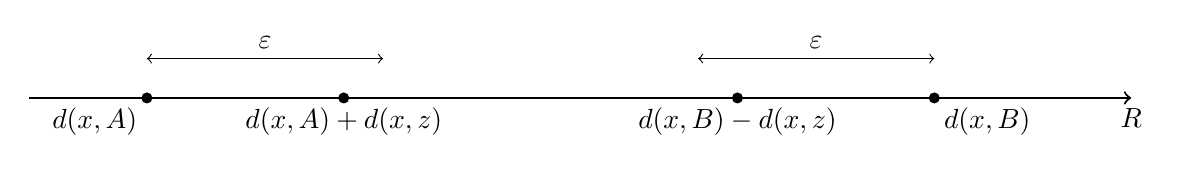
\begin{tikzpicture}
    % Draw the real line
    \draw[thick,->] (-0.5,0) -- (13.5,0) node[below] {$\mathbb{R}$};
    
    % Left Markers
    \fill (1,0) circle (2pt);
    \fill (3.5,0) circle (2pt);
    \node[below left] at (1,0) {$d(x,A)$};
    \node[below] at (3.5,0) {$d(x,A) + d(x,z)$};
    \draw[<->] (1,0.5) -- (4,0.5) node[midway,above] {$\varepsilon$};

    % Right Markers
    \fill (8.5,0) circle (2pt);
    \fill (11,0) circle (2pt);
    \node[below right] at (11,0) {$d(x,B)$};
    \node[below] at (8.5,0) {$d(x,B) - d(x,z)$};
    \draw[<->] (8,0.5) -- (11,0.5) node[midway,above] {$\varepsilon$};
\end{tikzpicture}
    \caption{Exercise 4.3: Finding a $\varepsilon$ small enough that fits within $d(x,A) < d(x,B)$}
    \label{fig:ex4.3}
\end{figure}
\end{proof}
\newpage

\exercise{4.4}
\begin{wts}
    
\end{wts}
\begin{proof}
    
\end{proof}
\newpage


\exercise{4.5}
\begin{wts}
    Every separable metric space is second countable.
\end{wts}
\begin{proof}
    We wish to show that if $\xx$ is a metric space, then
    \[
        \text{second countable } \iff \text{ separable}
    \]
    Suppose $\xx$ is separable, where $A$ is a countable dense subset in $\xx$, and $x\in\xx$. Let $U$ be an open set that contains $x$, so $B(\varepsilon,\: x)\subseteq U$ for some $\varepsilon>0$. $B(\varepsilon/2,\: x)$ is a non-empty open set, therefore contains some $y\in A$ (this follows from the definition of density). If we choose $r\in \mathbb{Q}$ wisely,
    \[
        d(x,y) < r < \varepsilon/2
    \]
    So that $x\in B(r,\: y)$, and if $z\in B(r,\: y)$, then 
    \[
        d(x,z)\leq d(x,y) + d(z,y)< r + r < \varepsilon
    \]
    So $x \in B(r,\: y)\subseteq U$. But $\{B(r,y),\: r\in\rat^+,\: y\in A\}$ is countable. Therefore $\xx$ is second countable.\\
    
    Conversely, Proposition 4.5 gives us the $\impliedby$ direction. But we will repeat anyway, if $\xx$ is second-countable with $\Epsilon$ as a countable base, then take 
    \[
        W = \bigset{x_\alpha\in U,\quad U\in \Epsilon}
    \]
    by picking a point from each set, we claim $W$ is dense in $\xx$, so $\cl{W}=\xx$. If not, then $\cl{W}^c \neq\varnothing$, and 
    \[
        \cl{W}^c = (W^c)^o \neq \varnothing
    \]
    Pick a point $x \in W^{co}$, which is an open set containing $x$. But the way we chose $W$ does not allow for any open set $U\in \Epsilon$ with $x\in\Epsilon \subseteq W^{co}$, since
    \begin{quote}
        By picking one point from each of the base sets, grouping these points and call it $W$, and flipping to the complement. Each $U\in\Epsilon$ admits a point that escapes $W^{co}$. Therefore we can ensure  no $U\in\Epsilon$ can be a subset of $W^{co}$. 
    \end{quote}
\end{proof}
\newpage

\exercise{4.6}
\begin{wts}
\end{wts}
\begin{proof}
    
\end{proof}
\newpage

\exercise{4.7}
\begin{wts}
    If $\xx$ is a topological space, a point $x\in\xx$ is called a cluster point of the sequence $\{x_j\}$ if for every neighbourhood $U\in\N{x}$, $x_j\in U$ for infinitely many $j$. If $\xx$ is first countable, $x$ is a cluster point of $\{x_j\}$ iff some subsequence of $\{x_j\}$ converges to $x$.
\end{wts}
\begin{proof}
    Suppose $\{x_n\}$ has a cluster point in $z\in \xx$. Fix a descending sequence of neighbourhoods $U_k\subseteq \N{z}$, where
    \[
        U_1\supseteq U_2\supseteq\cdots\supseteq U_k
    \]
    Define $n_k = \least\bigset{j\in \natplus,\: j>n_{k-1},\: x_j\in U_k}
    $ with $n_0=0$, so that for every $m\geq k$, $x_{n_m}\in U_k$ eventually. And $\{x_{n_j}\}_{j\geq 1}$ is a subsequence which converges to $z$. This proves ($\implies$).\\
    
    Conversely (this part does not require that $\xx$ be first countable), if $\{x_{n_k}\}_{k\geq 1}$ is a subsequence that converges to $z\in\xx$. Every neighbourhood of $z$ must intersect all but infinitely many $x_{n_k}$, therefore $z$ is a cluster point of $\{x_n\}$.
\end{proof}
\newpage




\exercise{4.8}
\begin{wts}
    If $\xx$ is an infinite set with the cofinite topology and $\{x_j\} $ is a sequence of distinct points in $\xx$, then $x_j\to x$ for every $x\in\xx$.   
\end{wts}
\begin{proof}
    The intuition here is that the cofinite topology does not distinguish between points, so it acts as a type of jelly that hides the points.\\

    Let $x\in\xx$ be arbitrary, if $U\in\N{x}$ then $U^o\in\N{x}$, so that $\{y_j\}_{j\leq k}$ are the $k$ points that are required to extend $U^o$ to $\xx$. (All but finitely many points are in any open set of $\xx$).\\

    There exists a large $N\in\natplus$ so that for every $n\geq N$, 
    \[
        x_j\notin\{y_j\}_{j\leq k}\implies x_j\in U^o
    \]
    eventually. And $x_j\to x$.
\end{proof}
\newpage

\exercise{4.9}
\begin{wts}
    
\end{wts}
\begin{proof}
    
\end{proof}
\newpage

\exercise{4.10}
\begin{wts}
    A topological space $\xx$ is called disconnected if there exists non-empty, disjoint open sets $U$, $V$ and $U\cup V = \xx$; otherwise $\xx$ is connected. When we speak of connected or disconnected subsets of $\xx$, we refer to the relative topology on them
    \begin{enumalpha}
        \item $\xx$ is connected iff $\varnothing$ and $\xx$ are the only two clopen sets.
        \item If $\{E_\alpha\}_{\alpha\in A}$ is a collection of connected subsets of $\xx$, and $bigcap E_{\alpha\in A}$ is non-empty, then $\bigcup E_{\alpha\in A}$ is connected.
        \item If $A\subseteq\xx$ is connected, then $\cl{A}$ is connected,
        \item Every point in $x\in\xx$ contained in a unique maximal connected subset of $\xx$, and this subset is closed. It is called the connected component of $x$.
    \end{enumalpha}
\end{wts}
\begin{proof}
    The proof is rather long, so we will split it in several parts. A topological space is disconnected iff it can be written as a disjoint union of two non-empty open sets. Often it is easier to show that a space is disconnected rather than connected.\\

    Part A: Suppose $\xx$ is disconnected, this induces a pair of non-empty open sets, $A$, and $B$ whose union is $\xx$, and 
    \[
        A\cap B = \varnothing\iff A \subseteq B^c
    \]
    their union is $\xx$, hence
    \[
        A\cup B = \xx\iff B^c\subseteq A
    \]
    combining the last two estimates, we see that $B = A^c$, so both $A$ and $A^c = B$ are closed. This proves ($\impliedby$).\\
    Now suppose $\{A, A^c\}\neq \{\varnothing,\xx\}$ are both clopen. Clearly $A$ is disjoint from its complement, and their union is $\xx$.\\

    Part B: We will attempt the contrapositive. Suppose $E = \bigcup E_{\alpha\in A}$ is disconnected. This induces $D$ and $D^c$ which are clopen in the relative topology of $E$, (by Part A). More precisely,
    \begin{equation}\label{chp4:ex4.10-union-non-empty}
        \bigcup E_\alpha = \underbrace{\bigcup (E_\alpha\cap D)}_{\neq\varnothing} + \underbrace{\bigcup (E_\alpha\setminus D)}_{\neq\varnothing}
    \end{equation}
    The intersection $\bigcap E_{\alpha\in A}$ is non-trivial, hence
    \begin{equation}\label{chp4:ex4.10-intersection-non-empty}
        \bigcap E_\alpha = \underbrace{\bigcap (E_\alpha\cap D)}_{\neq\varnothing} + \bigcap (E_\alpha\setminus D) \neq\varnothing
    \end{equation}    
    so at least one of the members on the right are non-empty. Assume without loss of generality that $\bigcap (E_\alpha\cap D)$ is not empty. This tells us $E_\alpha\cap D=\neq\varnothing$ for each $\alpha\in A$. But by \Cref{chp4:ex4.10-union-non-empty}, if we concentrate on the right member, 
    \[
        \bigcup (E_\alpha\setminus D)\neq\varnothing\implies\exists\beta\in A,\: E_\alpha\setminus D \neq\varnothing
    \]
    And for this particular $\beta\in A$, we see that both $D$ and $D^c$ are non-trivially open in $E_\beta$, and the proof is complete. A poetic way to summarize the proof would be:
    \begin{quote}
        If the whole is disconnected, and there exists common ground over which the family of sets covers, and because the common ground (intersection) is non-trivial, either $D$ or $D^c$ is non-trivially open in all $E_\alpha$. The intersection gives us "$\forall$", while the union gives us "$\exists$" for a non-trivially open $D$ or $D^c$.
    \end{quote}

    There is an alternate way of proving Part B, without using the clopen definition of connectedness. Let $C$ and $D$ be non-empty, disjoint, open sets in $\bigcup E_\alpha$ whose union is $\bigcup E_\alpha$. 
    \[
        \bigcap E_\alpha = \bigcap [E_\alpha\cap C] + \bigcap[E_\alpha\cap D]\neq\varnothing
    \]
    Pick $p\in\bigcap E_\alpha$, without loss of generality, assume $p\in\bigcap [E_\alpha\cap C]$, then for every $\alpha$ we have
    \[
        p\in E_\alpha\cap C\implies E_\alpha\cap C\neq\varnothing
    \]
    Since $E_\alpha$ is connected, $E_\alpha\cap D=\varnothing$ for each $\alpha$. Taking the union over all $E_\alpha\cap D$, we see that
    \[
        \bigcup [E_\alpha\cap D] = \varnothing
    \]
    which contradicts the assumption $D\neq\varnothing$.

    Part C: Suppose $\cl{A}$ is disconnected, this induces a non-trivial clopen set $D$ relative to $\cl{A}$. 
    \begin{itemize}
        \item Since $\cl{A}\cap D\neq\varnothing$, choose any $y\in\cl{A}\cap D\subseteq \cl{A}$, since $D$ is a neighbourhood of $y$, and $y$ is an adherent point of $A$. It is immediate that $A\cap D$ is non-empty.
        \item Similarly for $A\setminus D\neq\varnothing$,
    \end{itemize}
    therefore $\{D,D^c\}$ is non-trivially clopen in $A$, and $A$ is disconnected.\\

    Part D: The idea here is to use Part B. Let $x$ be fixed, and $\{E_\alpha\}_{\alpha\in A}$ be the family of all connected sets containing $x$, since their intersection is non-trivial, their union, $E$ is connected. The closure of their union is then the maximal connected component containing $x$. Indeed, if $G$ is a connected set containing $x$, then $G\subseteq \bigcup E_\alpha = E$, so $G\subseteq \cl{E}$.
\end{proof}
\newpage

\exercise{4.11}
\begin{wts}
    If $E_1,\ldots E_n$ are subsets of a topological space, the closure of $\bigcup_1^n E_j$ is $\bigcup_1^n \cl{E_j}$
\end{wts}
\begin{proof}
    The finite union of closed sets is again closed, so 
    \[
        \forall j\leq n,\: E_j\subseteq \cl{E_j}\implies \cl{\bigcup_1^n E_j}\subseteq \bigcup_1^n \cl{E_j}
    \]
    For the reverse estimate, $E_j\subseteq\bigcup_1^n E_j\subseteq \cl{\bigcup_1^n E_j}$ is a closed set that contains each $E_j$, therefore
    \[
        \forall j\leq n,\: \cl{E_j}\subseteq \cl{\bigcup_1^n E_j}\implies \bigcup_1^n \cl{E_j}\subseteq \cl{\bigcup_1^n E_j}
    \]
\end{proof}
\begin{corollary}
    The interior operator distributes over intersections. If $A$ and $B$ are subsets of $\xx$, then
    \begin{align*}
        \cl{(A^c\cup  B^c)} &= (\cl{A^c}\cup \cl{B^c})\\
        \biggl(\cl{(A^c\cup  B^c)}\biggr)^c&= A^o\cap B^o\\
        \biggl(A^c\cup B^c\biggr)^{co} &= A^o\cap B^o\\
        (A\cap B)^o&=A^o\cap B^o
    \end{align*}
\end{corollary}
\newpage

% Kuratowski Closure Operaotrs
\exercise{4.12}
\begin{wts}
    Let $\xx$ be a set. A Kuratowski closure operator on $\xx$ is a map $A\mapsto A^*$ from $\powerset{\xx}$ to itself satisfying
    \begin{enumroman}
        \item $\varnothing^* = \varnothing$ (does nothing to the empty set),
        \item $A\subseteq A^*$ (monotonicity),
        \item $(A^*)^* = A^*$ (idempotence)
        \item $(A\cup B)^* = A^* \cup B^*$ (distributes over finite unions)
    \end{enumroman}
    Prove
    \begin{enumalpha}
        \item If $\xx$ is a topological space, the map $A\mapsto \cl{A}$ is a Kuratowski closure operator. (Use Exercise 11.)
        \item Conversely, given a Kuratowski closure operator, let $\mathcal{F} = \{ A\subseteq \xx,\: A = A^*\}$ and $\Tau = \{U\subseteq \xx,\: U^c\in \mathcal{F}\}$, then $\Tau$ is a topology on $\xx$, and for any set $A\subseteq\xx$, $A^*$ will be its closure with respect to $\Tau$.
    \end{enumalpha}
\end{wts}
\begin{proof}
    Part A: The empty set is closed, so $\cl{\varnothing}=\varnothing$, and $\cl{A}$ is the smallest closed superset of $A$, so $A\subseteq\cl{A}$ for every $A\subseteq\xx$. $A\subseteq\xx$ is closed iff $\cl{A} = A$, so idempotence holds. Distributivity follows from Exercise 11 directly.\\

    Part B: We first show that $\Tau$ is indeed a topology. Fix $U_1$ and $U_2$ in $\Tau$, so that $U_1^c\cup U_2^c = (U_1\cap U_2)^c$. The map $A\mapsto A^*$ distributes over finite unions, hence 
    \[
        (U_1^c \cup U_2^c)^* = (U_1^c)^* \cup (U_2^c)^* = U_1^c\cup U_2^c
    \]
    Therefore $U_1\cap U_2\in \Tau$. Now suppose $\{U_\alpha\}_{\alpha\in A}\subseteq\Tau$, then
    \[
        \biggl( \bigcup U_\alpha\biggr)^c = \bigcap U_\alpha^c
    \]
    by monotonicity (Property ii): $\bigcap U_\alpha^c\subseteq\biggl(\bigcap U_\alpha^c\biggr)^*$. To prove the reverse inclusion, notice if $\alpha$ is held fixed,
    \[
        \bigcap U_\alpha^c\subseteq U_\alpha^c\implies \biggl(\bigcap U_\alpha^c\biggr)^*\subseteq U_\alpha^{c*}
    \]
    this follows from 'monotonicity' of the closure operator: if $A$ is a subset of $B$, then we can write 
    \[
        B = A + (B\setminus A)\implies A^* \subseteq A^* + (B\setminus A)^* = B^*
    \]
    Take the intersection over all $\alpha\in A$ on the right member,
    \[
        \biggl(\bigcap U_\alpha^c\biggr)^*\subseteq \bigcap U_\alpha^{c*} = \bigcap U_\alpha^c
    \]
    Hence $\biggl(\bigcap U_\alpha^c \biggr)^* = \bigcap U_\alpha^c $. The empty set and $\xx$ are elements of $\mathcal{F}$. Since $\xx\subseteq \xx^*\subseteq \xx$, and $\{\varnothing,\xx\}\subseteq\Tau$. So $\Tau$ is a topology.\\

    Finally, $A^*$ is a closed superset of $A$ and suppose $K$ is another closed superset,
    \[
        A \subseteq K\implies A^*\subseteq K^*
    \]
    So $A^*$ is the smallest closed superset of $A$ and this proves the last claim.
\end{proof}
\newpage




\exercise{4.13}
\begin{wts}
    If $\xx$ is a topological space, $U$ is open in $\xx$ and $A$ is dense in $\xx$, then $\cl{U} = \cl{U\cap A}$.
\end{wts}
\begin{proof}
    The takeaway here is that if $A$ is dense in $\xx$, every point $z\in U$ can be approximated by points in $U\cap A$. And and important technique of 'demoting' the neighbourhood to become the interior of the neighbourhood can yield some nice properties. Since the interior of a neighbourhood is again a neighbourhood. This allows intersection with open sets to inherit the 'neighbourhoodness' of the set.\\

    Let $z\in \cl{U}$, and fix a neighbourhood $V\in \N{z}$, so that the interior of $V$ is also a neighbourhood. By the alternate definition of $\cl{U}$ in terms of adherent points (see \Cref{chp4:closure-adherent}) of $\cl{U}$, $V^o\cap U\neq\varnothing$. This is a non-empty open set, therefore it must intersect $A$ non-trivially.
    \[
        x\in (V^o\cap U)\cap A = V^o\cap (U\cap A)
    \]
    and $z\in \cl{U\cap A}$.\\
\end{proof}
\begin{remark}
We simply used the fact 
\[
\cl{E} = \bigset{x\in\xx,\: \forall V\in\N{x},\: V\cap E\neq\varnothing}
\]
and the following equivalent characterization of density
\[
E \text{ is dense in }\xx \iff \text{ For every non-empty open set } U,\: U\cap E\neq\varnothing
\]
\end{remark}
\newpage


\exercise{4.14}
\begin{wts}
    If $\xx$ and $\yy$ are topological spaces, $f: \xx\to\yy$ is continuous iff $f(\cl{A})\subseteq\cl{f(A)}$ for every $A\subseteq \xx$ iff $\cl{f^{-1}(B)}\subseteq f^{-1}(\cl{B})$ for all $B\subseteq Y$.
\end{wts}
\begin{proof}
    \emph{First Equivalence:} If $f$ is continuous, fix any $A\subseteq\xx$, and $z\in \cl{A}$, by \Cref{chp4:closure-adherent} (I will spare you the flipping by including):
    \[
    \cl{A} = \{x\in\xx,\: \forall U\in\N{X},\: U\cap A\neq\varnothing\}
    \]
    Let $U\in \N{f(z)}$, so that $f^{-1}(U^o)$ is an open set containing $z$ and $f^{-1}(U^o)\in\N{z}$, so
    \[
        f^{-1}(U^o)\cap A\neq\varnothing\implies U^o\cap f(A)\subseteq U\cap f(A)
    \]
    so $f(\cl{A})\subseteq \cl{f(A)}$. Conversely, suppose $f(\cl{A})\subseteq\cl{f(A)}$ holds for every $A\subseteq\xx$. The following is a sequence of symbolic manipulations that I found but have zero intuitive understanding about. First take the inverse image
    \[
        \cl{A}\subseteq f^{-1}\biggl(f(\cl{A})\biggr)\subseteq f^{-1}\biggl(\cl{f(A)}\biggr)
    \]
    Next, let $F$ be a closed set in $\yy$, and make the substitution $A = f^{-1}(F)$, hence
    \[
        \cl{f^{-1}(F)}\subseteq f^{-1}\biggl(\cl{f(f^{-1}(F))}\biggr)\subseteq f^{-1}(\cl{F})=f^{-1}(F)
    \]
    for the second inclusion we used the monotonicity of the closure, and since $\cl{f^{-1}(F)} = f^{-1}(F)$, we are done.
    \\

    \emph{Second Equivalence:} Suppose $f\in C(\xx,\yy)$, then $\cl{B}\subseteq \yy$ is a closed set, so $f^{-1}(\cl{B})$ is closed in $\xx$. By monotonicity of the inverse image,
    \[
        f^{-1}(B)\subseteq f^{-1}(\cl{B})\implies \cl{f^{-1}(B)}\subseteq f^{-1}(\cl{B})
    \]
    Conversely, if $\cl{f^{-1}(B)}\subseteq f^{-1}(B)$ for any $B\subseteq \yy$, take any closed $B\subseteq \yy$, and 
    \[
        \cl{f^{-1}(B)}\subseteq f^{-1}(B)\subseteq \cl{f^{-1}(B)}
    \]
    so $f^{-1}(B)$ is closed, and $f$ is in $C(\xx,\yy)$.
\end{proof}
\newpage


\exercise{4.16}
\begin{wts}
\end{wts}

\begin{proof}
    \begin{enumalpha}
        \item[]
        \item Let $x\in \{f\neq g\}$, then there exists disjoint open subsets of $\yy$, $f(x)\in U$ and $g(x)\in V$, $U\cap V=\varnothing$, but $f^{-1}(U)\cap g^{-1}(V)$ is an open set in $\xx$ that contains $x$. Therefore $\{f\neq g\}$ is open in $\xx$.
        \item Suppose $\{f=g\}=E$ is dense in $\xx$. Let $x\in E$, induces two disjoint open sets exactly like in part a. This is an open set that contains $x$, and $y\in f^{-1}(U)\cap g^{-1}(V)\cap E$. Since $y\in E$, it follows that $f(y) = g(y)$, and
        \[
            \begin{cases}
            y\in f^{-1}(U)\implies &f(y)\in U\\
            y\in g^{-1}(V)\implies &g(y)\in V
            \end{cases}
        \]
    \end{enumalpha}
\end{proof}
\newpage


\exercise{4.17}




\end{document}